\documentclass{article}
\usepackage[T2A]{fontenc}
\usepackage{fontspec}
\setmainfont{CMU Serif}
\usepackage{amsmath}
\usepackage{amssymb}
\usepackage[russian]{babel}
\usepackage{graphicx}
\usepackage{xeCJK}% 调用 xeCJK 宏包
\setCJKmainfont{SimHei}

\begin{document}
\author{Сюй Минчуань}
\title{Обзор комплексного анализа}
\maketitle
\tableofcontents
\newpage
\section{Основные понятия и элементарные функции}
\subsection{Дифференцируемость функций комплексной переменной. Условия Коши-Римана. Аналитичность. Вопрос 1 Лек.2}
	Пусть $ f $ - функция комплексного переменного, определённая и однозначная на некотором множестве $\mathbf{E}$, и пусть ${z}_{0}$ - какая-либо точка этого множества, являющаяся предельной для него.
	Если существует предел
	\begin{equation}
	\lim _{E \ni z \rightarrow z_{0}} \frac{f(z)-f\left(z_{0}\right)}{z-z_{0}}
	\end{equation}
	то он называется \textbf{производной функции} $ f $ по множеству $ E $ в точке $ z_{0} $ и обозначается через $ f^{\prime}\left(z_{0}\right) $. Сама функция $ f$, обладающая производной называется \textbf{дифференцируемой} или моногенной по Множеству $Е$ в точке $z_{0}$.\\
	\textbf{Критерий дифференцируемости} Функция $f$ тогда и только тогда дифференцируема в точке $z_{0}$, когда её приращение в этой точке можно представить в виде
	\begin{equation}
	\Delta f(z)=A\cdot \Delta z+\alpha({z}_{0},\Delta z)\cdot \Delta z
	\end{equation}
	где $A$ - константа, а $\alpha({z}_{0},\Delta z)$ бесконечная малая при $z\rightarrow {z}_{0}$. Если такое представление возможно, то $A=f'({x}_{0})$.\\
	\textbf{Условия Коши-Римана} Функция $ f(z)=u(x, y)+i v(x, y)$,  определённая в области $ \mathbf{G}$,  тогда и только тогда дифференцируема в точке $ z_{0}=x_{0}+iy_{0}$ этой области, когда функции $ u(x, y) $ и $ v(x, y) $ дифференцируемы в точке $ \left(x_{0}, y_{0}\right) $ и их частные производные в этой точке удовлетворяют соотношениям
	\begin{equation}
	u_{x}^{\prime}=v_{y}^{\prime}, \quad u_{y}^{\prime}=-v_{x}^{\prime}
	\end{equation}
	\\ 
	\textbf{Определение 1} Функция $ f$, дифференцируемая в каждой точке области $\mathbf{G}$, называется дифференцируемой или \textbf{аналитической} в этой области.\\
	\textbf{Определение 2} Если функция $ f $ дифференцируема в каждой точке области $\mathbf{G}$, a ee производная непрерывна в этой области, то $ f $ называется \textbf{аналитической} в $\mathbf{G}$.\\
	Эти определения эквивалентны, для удобства в дальнейшем мы будем использовать Определение 2. Обозначение: $f\in \mathcal{A}(\mathbf{G})$.\\
	Функция $f$ аналитична на всей плоскости $\mathbb{C}$ называется \textbf{целыми (аналитическими) функциями}.\\
\subsection{Свойства аналитических функций. Геометрический смысл производной. Вопрос 6 Лек.2}
	\textbf{Свойства аналитических функций}\\
	1) $ f \in \mathcal{A}(\mathbf{G}) \Rightarrow f \in \mathcal{C}(\mathbf{G})$.\\
	2) Пусть $ f_{1}, f_{2} \in \mathcal{A}(\mathbf{G}) $. Тогда сумма, разность и произведение функций $ f_{1} $ и $ f_{2} $ также являются аналитическими функциями в $\mathbf{G}$. Функция $\varphi=\frac{f_{1}}{f_{2}}$ аналитична всюду, где $ f_{2}(z) \neq 0$.\\
	3) \textbf{Теорема об образе области} Пусть $ f \in \mathcal{A}(\mathbf{G})$ и $f\ne const$. Тогда множество $\mathbf{D}=f(\mathbf{G})$ также является областью.\\
	4) \textbf{Аналитичность сложной функции} Пусть $ f(z) \in \mathcal{A}(  G  ) $ и $f(z) \neq  const$. Ecли в области $ \mathbf{D}=f(\mathbf{G}) $ определена аналитическая функция $ \zeta=g(w)$, $ то функция  \zeta=g(f(z)) \equiv H(z) $ является аналитической функцией переменной $z$ в области $\mathbf{G}$.\\
	5) \textbf{Аналитичность обратной функции} Пусть $ f(z) \in \mathcal{A}(  G  ) $ и $f'({z}_{0}) \neq  0$ в некоторой точке ${z}_{0}\in \mathbf{G}$. Положим $ w_{0}=f\left(z_{0}\right) $. Тогда найдутся окрестность $ K_{\varepsilon} $ точки $ w_{0} $ и функция $ z=\varphi(w) $ такие, что:\\
	1. Функция $ \phi $ обратна k $f$, т.е. $f[\phi(w)]=w \quad \forall w \in K_{\varepsilon}$,\\
	2. $\phi(w) \in \mathcal{A}\left(K_{\varepsilon}\right)$,\\ 
	3. производную $ \phi^{\prime}\left(w_{0}\right) $ можно вычислить по хорошо известной формуле $\phi^{\prime}\left(w_{0}\right)=\frac{1}{f^{\prime}\left(z_{0}\right)}$.\\
	6) \textbf{Ортогональность линий уровня} Линии уровня разных семейств в каждой точке области $\mathbf{G}$ ортогональны.\\
	\\
	\textbf{Геометрический смысл аргумента производной} Число $\arg  f^{\prime}\left(z_{0}\right) $ есть угол поворота всякой гладкой кривой, проведённой через точку $ z_{0}$,  при переходе от плоскости $ z $ к плоскости $ w $.  Этот поворот происходит под действием функции $ f $.
	\\
	\textbf{Локальная конформность} Отображение посредством непрерывной функции, сохраняющее углы между кривыми, проходящими через данную точку, называется \textbf{конформный в этой точке}.\\
	\textbf{Глобальная конформность} Пусть функция $f$ отображает область $\mathbf{G}$ в $\mathbf{D}$ взаимно однозначно. Если при этом $f$ конформна в каждой точке $z\in \mathbf{G}$, то говорят, что $f$ отображает $\mathbf{G}$ в $\mathbf{D}$ \textbf{конформно}.\\
	\textbf{Достаточное условие локальной конформности} Отображение конформно во всех точках ${z}_{0}$, где $f'({z}_{0})\ne 0$.\\
\subsection{Дробно-линейные функции: инвариантность двойного отношения,  круговое свойство. Вопрос 5 Лек.3}
	\begin{equation}
	w=L(z)=\frac{a z+b}{c z+d}
	\end{equation}
	При этом не должно быть равно нулю число
	\begin{equation}
	\delta=a d-b c=\operatorname{det}\left|\begin{array}{ll}
	a & b \\
	c & d
	\end{array}\right|
	\end{equation}
	называемое \textbf{определителем} функции $L$.\\
	\\
	\textbf{Инвариантность двойного отношения}\\
	Пусть $ a, b, c, d$ - конечные и попарно различные комплексные числа. Их \textbf{двойным (или ангармоническим) отношением} называется число
	\begin{equation}
	(a, b, c, d)=\frac{c-a}{c-b}: \frac{d-a}{d-b}
	\end{equation}
	\textbf{Теорема. Двойное отношение есть инвариант дробно-линейного преобразования}
	Пусть $ w=L(z)$ - произвольная дробно-линейная функция, $ a, b, c, d$ - произвольные конечные и попарно различные числа, $ A, B, C, D$ - их образы под действием функции $ L(z) $. Утверждается, что
	\begin{equation}
	(a, b, c, d)=(A, B, C, D)
	\end{equation}
	\\
	\textbf{Теорема. Kруговое свойство} Образ прямой или окружности при дробно-линейном преобразовании есть прямая или окружность.\\
	\textbf{Замечание} Если прямая или окружность (не) проходит через особую точку $ \delta=-d / c $ дробно-линейной функции $ L(z)$, то ее образ под действием этой функции (не) должен содержать точку $ \infty=L(\delta) $ и, следовательно, является прямой (окружностью). 
\subsection{Сохранение симметрии. Примеры типовых дробно-линейных отображений. Вопрос 7 Лек.4}
	Говорят, что точки $ z_{1} $ и $ z_{2} $ \textbf{симметричны относительно окружности} $ \gamma $, если прямая и всякая окружность, проходящие через ${z}_{1}$ и $ z_{2} $ ортогональны $ \gamma $ (см. слайд "Симметрия относительно окружности ").\\
	Пусть $\gamma$ задана уравнением $|z-a|=R$, тогда справедливо
	\begin{equation}
	{z}_{2}=a+\frac{{R}^{2}}{\overline{{z}_{1}-a}}
	\end{equation}
	\textbf{Теорема} Под действии произвольного дробно-линейного преобразования $w=L(z)$ точки ${z}_{1}$ и ${z}_{2}$, симметричные относительно прямой или окружности $\gamma$, переходят в точки ${w}_{1}$ и ${w}_{2}$, симметричные относительно прямой или окружности $\Gamma=L(\gamma)$.\\
	\\
	\textbf{Пример}\footnote{Подробнее объяснение см. стр.70-72} Построить дробно-линейное преобразование $ w=L(z)$, преобразующее круг $ |z|<R $ в круг $ |w|<R $ так, чтобы заданная точка $ \alpha $ первого круга перешла в центр $ w=0 $ второго круга. Рассмотрим два возможных случая.\\
	1) $\alpha=0$, тогда решение будет целая линейная функция вида $w={e}^{i\phi}z$, где $\phi$ - произвольное число из $[0,2\pi)$.\\
	2) $\alpha\ne0$, тогда решение будет дробно-линейная функция вида $w={R}^{2}{e}^{i\phi}\frac{z-\alpha}{{R}^{2}-\overline{\alpha}z}$.\\
\subsection{Функция Жуковского. Вопрос 20}
	\textbf{Функция Жуковского}
	\begin{equation}
	w=\lambda(z)=\frac{1}{2}(z+\frac{1}{z}), dom\,\lambda=\mathbb{C}\setminus \{0\},im\,\lambda=\mathbb{C}
	\end{equation}
	Функция Жуковского имеет непрерывную производную, и поэтому $\lambda(z)$ аналитична в $dom\,\lambda$, обладает свойством локальной комформности, но не обладает глобальной комформности. Она двулистна\footnote{Определения см. стр.75} в своей области определения. Её областью однолистности является 1) единичный круг $|z|<1$, 2) область $|z|>1$, 3) полуплоскость $\operatorname{Im}z<0$ и 4) полуплоскость $\operatorname{Im}z>0$.\\
	\\
	\textbf{Типичные преобразования Функции Жуковского}\\
	1) Семейство окружностей
	\begin{equation}
	{\gamma}_{r}:z=r(\cos t+i\sin t),t\in [0,2\pi],r\in (0,1)
	\end{equation}
	переходит в объединение софокусных(точки -1 и 1) эллипсов
	\begin{equation}
	{\Gamma}_{r}:w=\frac{1}{2}(r+\frac{1}{r})\cos t-i\frac{1}{2}(r-\frac{1}{r})\sin t,t\in [0,2\pi],r\in (0,1)
	\end{equation}
	То есть
	\begin{equation}
	|z|<1\xrightarrow[\text{конформно}]{\lambda(z)}\mathbb{C}\setminus \{(u,v):-1\le u\le1,v=0\}
	\end{equation}
	2) Аналогично,
	\begin{equation}
	\begin{aligned}
	&\underbrace{\{z:|z|<1,Im z>0\}}_{\textbf{верхняя половина единичного круга}}\xrightarrow[\text{конформно}]{\lambda(z)} Im z<0\\
	&\underbrace{\{z:|z|>1,Im z<0\}}_{\textbf{нижняя полуплоскость кроме верхнего полукруга}}\xrightarrow[\text{конформно}]{\lambda(z)} Im z<0\\
	&\underbrace{\{z:|z|<1,Im z<0\}}_{\textbf{нижняя половина единичного круга}}\xrightarrow[\text{конформно}]{\lambda(z)} Im z>0\\
	&\underbrace{\{z:|z|>1,Im z>0\}}_{\textbf{верхняя полуплоскость кроме верхнего полукруга}}\xrightarrow[\text{конформно}]{\lambda(z)} Im z>0
	\end{aligned}
	\end{equation}
	3) ${P}^{+}=Imz>0,{P}^{-}=Imz<0$ - верхнюю или нижнюю полуплоскость переходит в $\mathbb{C}\setminus (-\infty,-1]\bigcup [1,+\infty)$.\\
	4) Семейство радиусов единичного круга 
	\begin{equation}
	{r}_{\alpha}:z=t(\cos \alpha+i\sin \alpha),t\in (0,1),\alpha\in[0,2\pi]
	\end{equation}
	переходит в софокусных(точки -1 и 1) гиперболов
	\begin{equation}
	{R}_{\alpha}:w=\frac{1}{2}(t+\frac{1}{t})\cos \alpha-i\frac{1}{2}(t-\frac{1}{t})\sin \alpha,t\in (0,1),\alpha\in[0,2\pi]
	\end{equation}
	\begin{figure}
		\centering
		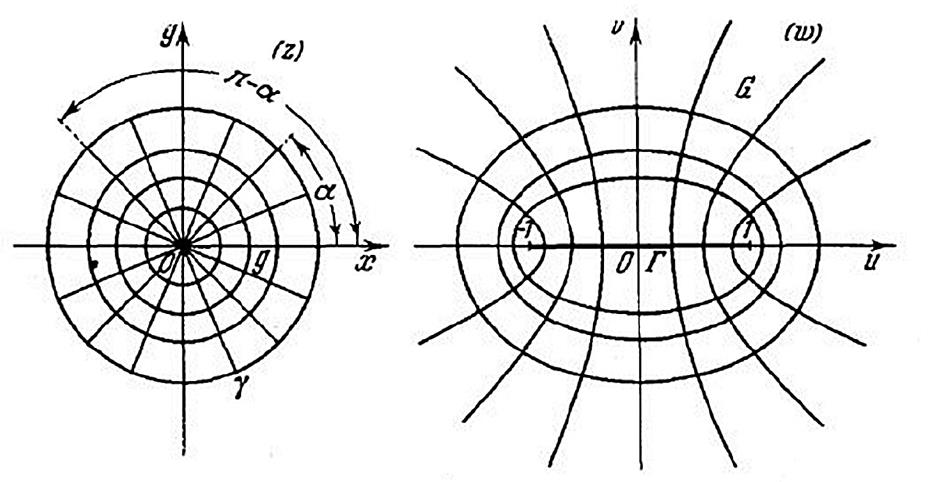
\includegraphics[width=0.7\linewidth]{fig1}
		\caption{Конформное действие функции Жуковского в единичном круге}
		\label{fig:fig1}
	\end{figure}
	
\subsection{Показательная функция. Тригонометрические и гиперболические функции. Вопрос 14 Лек.5}
	\textbf{Показательная функция} Пусть $z=x+iy$, то
	\begin{equation}
	{e}^{z}={e}^{x}(\cos x+i\sin y), dom\,{e}^{z}=\mathbb{C},im\,{e}^{z}=\mathbb{C}\setminus \{0\}
	\end{equation}
	Эта функция аналитична во всей комплексной плоскости и $2\pi i$ периодична, обладает локальной и глобальной конформности в любой точке плоскости. Всякая горизонтальная полоса $g:{\phi}_{0}<y<{\phi}_{1}$ ширины $h={\phi}_{1}-{\phi}_{0}\le 1\pi$ является областью однолистности
	Каждое число $w$ из образа функции имеет прообразы вида $z=\ln|w|+iArg\,w$. Каждое из этих чисел назывется \textbf{(натуральным) логарифмом} числа $w$. Все они расположены на одной и той же вертикальной прямой $x=\ln|w|$, и расстояние между соседними равно $2\pi i$.\\
	\\
	\textbf{Типичные преобразования показательной функции}\\
	1) Горизотальная прямая
	\begin{equation}
	{I}_{\phi}:z=t+i\phi,-\infty<t<+\infty,{\phi}_{0}<\phi<{\phi}_{1}
	\end{equation}
	переходит в луч
	\begin{equation}
	{L}_{\phi}:w={e}^{t}(\cos \phi+i\sin \phi),-\infty<t<+\infty,{\phi}_{0}<\phi<{\phi}_{1}, -\infty<t<+\infty,{\phi}_{0}<\phi<{\phi}_{1}
	\end{equation}
	Таким образом, горизотальная полоса $g$ переходит в сектор $G$ раствора $h$ с вершиной в точке $w=0$. Граничные лучи этого сектора задаются уравнениями $Arg\,w={\phi}_{0}+2k\pi$ и $Arg\,w={\phi}_{1}+2k\pi$. То есть
	\begin{equation}
	g\xrightarrow[\text{конформно}]{exp\,z} G
	\end{equation}
	2) Вертикальная прямая
	\begin{equation}
	{I}_{c}:z=c+it,-\infty<t<+\infty
	\end{equation}
	переходит в окружность
	\begin{equation}
	\gamma_{c}:w={e}^{c}(\cos t+i\sin t)
	\end{equation}
	Каждому отрезку длины $2\pi$ на прямой ${I}_{c}$ соответствует один обход $\gamma_{c}$.\\
	3) Прямая, не параллельная вещественной и мнимой осям, отображается экспонентой в логарифмическую спираль (кривую, задаваемую полярным уравнением $ \rho=C e^{k \phi}$, где $ C>0 $ и $ k$ - константы).\\
	\\
	\textbf{Тригонометрические и гиперболические функции} Мы определим таких функции:
	\begin{equation}
	\begin{aligned}
	\cos z=\frac{e^{i z}+e^{-i z}}{2}, &\sin z=\frac{e^{i z}-e^{-i z}}{2 i} \\
	\operatorname{ch} z=\frac{e^{z}+e^{-z}}{2}, &\operatorname{sh} z=\frac{e^{z}-e^{-z}}{2}\\
	\operatorname{tg} z=\frac{\sin z}{\cos z}, &\operatorname{ctg} z=\frac{\cos z}{\sin z}\\
	\operatorname{th} z=\frac{\operatorname{sh} z}{\operatorname{ch} z}, &\operatorname{cth} z=\frac{\operatorname{ch} z}{\operatorname{sh} z} 
	\end{aligned}
	\end{equation}
	Первые четыри функции, будучи линейными комбинациями экспонент, являются целыми и наследуют от них периодичность. При этом $\operatorname{sh} z$ и $\operatorname{ch}z$ имеют тот же период $2  \pi  i$. Tригонометрические функции $\sin z$ и $\cos z$ имеют период $ 2 \pi$. Последние четыри являются аналитическими всюду, где определены и периодичны, причем $\operatorname{th} z$ и $\operatorname{cth}z$ имеют период $\pi i$, a $\operatorname{tg} z$ и $\operatorname{ctg}z$ - период $ \pi $. \\ 
	$\sin z$ и $\cos z$ в нуль не обращаются вне вещественной оси, и они неограничены на плоскости.\\
	Все эти функции могут быть представлены композициями ранее функций: дробно-линейных, функции Жуковского и экспонет.\\
\section{Интегралы по комплексным переменным}
\subsection{Интегральная теорема Коши и её обобщения. Вопрос 11 Лек.6}
	\textbf{Теорема Жордана} Всякая замкнутая жорданова кривая $\Gamma$ делит плоскость $\mathbb{C}$ на две различные области, общей границей которых она является. При этом одна из областей ограничена. Она называется \textbf{внутренностью} $\Gamma$ и обозначается int $ \Gamma $ (oт interior). Вторая область не ограничена, называется \textbf{внешностью} $ \Gamma $ и обозначается ext $ \Gamma $ (от exterior).\\
	\textbf{Формула Грина} Пусть область $ D $ ограничена контуром $ C$, а функции $ P(x, y) $ и $ Q(x, y) $ непрерывны в замкнутой области $ D $ и имеют в $ D $ непрерывные частные производные $ \frac{\partial Q}{\partial x} $ и $ \frac{\partial P}{\partial y} $. Тогда справедлива \textbf{формула Грина}
	\begin{equation}
	\int_{C^{+}} P d x+Q d y=\iint_{\bar{D}}\left(\frac{\partial Q}{\partial x}-\frac{\partial P}{\partial y}\right) d x d y
	\end{equation}
	при условии, что двойной интеграл в правой части существует хотя бы как несобственный.\\
	\textbf{Интегральная теорема Коши} Пусть $f(z)=u(x,y)+iv(x,y)\in \mathcal{A}(\mathbf{G})$. Если $C$ - любой контур, принадлежащий области $\mathbf{G}$ вместе со своей внутреннстью, то
	\begin{equation}
	\oint_{C}f(z)dz=0
	\label{cauchy}
	\end{equation}
	\textbf{Следствие} Пусть $G$ - односвязная\footnote{Это существенное условие, см. стр.112} область и $ f(z) \in \mathcal{A}(\mathbf{G}) $. Тогда равенство \ref{cauchy} имеет место для любого контура $ C \subset  G$.\\
	\\
	\textbf{Обобщённая теорема Коши} Пусть $ \mathbf{G}$ - область, ограниченная контуром $ C $. Если функция $ f(z) \in \mathcal{A}(\mathrm{G}) $ сохраняет непрерывность на границе области, то
	\begin{equation}
	\oint_{C} f(z) d z=0
	\end{equation}
	\textbf{Составным контуром} называется объединение $ C=C_{0} \cup C_{1} \cup \cdots \cup C_{n} $ обычных (\textbf{простых}) контуров такое, что:\\
	1) Kонтур $C_{0}$, называемый \textbf{внешним}, содержит внутри себя все oстальные (\textbf{внутренние}) контуры $C_{1}, \ldots, C_{n}$.\\ 
	2) Kаждый из контуров $ C_{1}, \ldots, C_{n} $ лежит во внешности любого другого внутреннего контура.\\
	\textbf{Теорема о составном контуре} Пусть $ G$ - область, ограниченная составным контуром $ C=C_{0} \cup C_{1} \cup \cdots \cup C_{n} $. Если функция $ f(z) \in A(G) $ сохраняет непрерывность на границе области, то
	\begin{equation}
	\oint_{C^{+}} f(z) d z=\oint_{C_{0}^{+}} f(z) d z+\oint_{C_{1}^{-}} f(z) d z+\cdots+\oint_{C_{n}^{-}} f(z) d z=0
	\end{equation}
	Чаще всего используется такая формулировка:
	\begin{equation}
	\oint_{C^{+}} f(z) d z=\oint_{C_{0}^{+}} f(z) d z+\cdots+\oint_{C_{n}^{+}} f(z) d z
	\end{equation}
	
\subsection{Неопределённый интеграл и теорема о первообразной. Вопрос 21 Лек.7}
	Пусть $ f \in \mathcal{C}(\mathbf{G}) $. Функция $ \Phi \in \mathcal{A}(\mathbf{G}) $ называется \textbf{первообразной} функции $ f $ в этой области, если $\Phi'(z)=f(z)$. Cовокупнсть первообразных функции $ f$ в данной области называется её \textbf{неопределенным интегралом} в этой области.\\
	\textbf{Теорема о первообразной}\footnote{Теорема об эквивалентности трех высказывания см. стр. 122-123} Пусть $ f \in \mathcal{C}(\mathbf{G})$, и пусть для $ f $ имеет место $ C$ - свойство\footnote{$\oint_{L}f(z)dz=0$, где $L\subset \mathbf{G}$. см. стр.123} в $ \mathbf{G} $. Последнее корректно определяет интеграл $F(z)=\int_{{z}_{0}}^{z} f(\zeta)d\zeta$ как функцию только от верхнего предела $z$. Тогда:\\
	(A) $F \in \mathcal{A}(G)$ \\
	(B) $ F^{\prime}(z)=f(z) \forall z \in \mathbf{G}$ \\
	\\
	\textbf{Формула Коши} Пусть $ f \in \mathcal{A}(\mathbf{G})$, контур $ L \subset \mathbf{G}$, подобласть $ \mathbf{D} \subset \mathbf{G} $ ограничена контуром $ L $. Тогда для всякой точки $ z_{0} \in \mathbf{D} $ справедлива \textbf{формула Коши}.
	\begin{equation}
	f\left(z_{0}\right)=\frac{1}{2 \pi i} \oint_{L} \frac{f(z) d z}{z-z_{0}}
	\end{equation}
	\textbf{Формула среднего значения} Пусть $ \mathbf{G}$ - круг радиуса $ R $ с центром в точке $ z_{0} $, $ f \in \mathcal{A}(\mathbf{G})$ и $ f$ сохраняет непрерывность на границе области $\partial{G}=L$. Принимая для $ L $ параметризацию $ z=z_{0}+R e^{i \phi}$, получаем по формуле Коши
	\begin{equation}
	f\left(z_{0}\right)=\frac{1}{2 \pi i} \int_{0}^{2 \pi} \frac{f\left(z_{0}+R e^{i \phi}\right)}{R e^{i \phi}} i R e^{i \phi} d \phi=\frac{1}{2 \pi} \int_{0}^{2 \pi} f\left(z_{0}+R e^{i \phi}\right) d \phi
	\end{equation}
\subsection{Дифференцирование интеграла по параметру. Бесконечная дифференцируемость аналитических функций. Вопрос 8 Лек.8}
	Mы будем в дальнейшем рассматривать комплексные интегралы вида
	\begin{equation}
	F(z)=\int_{L} \phi(z, \zeta) d \zeta
	\end{equation}
	при следующих предположениях:\\
	(1)  $L$ - кривая на плоскости переменного $ \zeta=\xi+i \eta$, а $z$ изменяется в некоторой области $\mathbf{G}$ на плоскости переменного $ z=x+iy$.\\
	(2) При любом фиксированном значении $ \zeta \in L $ функция $\phi(z, \zeta)$ - аналитическая в области $\mathbf{G}$.\\
	(3) Функции $ \phi(z, \zeta) $ и $ \phi_{z}^{\prime}(z, \zeta) $ непрерывны по совокупности переменных $ z $ и $ \zeta $.\\
	\\
	\textbf{Теорема об интеграле с параметром} Пусть выполнены предположения (1)-(3). Тогда: \\
	1) интеграл $ F(z) \in \in \mathcal{A}(\mathbf{G})$;\\
	2) производную $ F^{\prime}(z) $ можно вычислить по правилу Лейбница:
	\begin{equation}
	F^{\prime}(z)=\int_{L} \phi_{z}^{\prime}(z, \zeta) d \zeta
	\end{equation}
	\\
	\textbf{Теорема о бесконечной дифференцируемости аналитической функции} Пусть $ f \in \mathcal{A}(\mathbf{G}) $. Тогда в каждой точке $ z \in \mathbf{G} $ функция $ f $ имеет производные всех порядков. Если контур $L$ принадлежит $\mathbf{G}$ вместе со своей внутренностью и $ z$ - внутренняя точка этого контура, то производная $ f^{(n)}(z) $ может быть вычислена по формуле
	\begin{equation}
	f^{(n)}(z)=\frac{n !}{2 \pi i} \oint_{L} \frac{f(\zeta)}{(\zeta-z)^{n+1}} d \zeta
	\end{equation}
	\textbf{Следствие} Производная аналитической функции сама является аналитической функцией.
\subsection{Теоремы Морера и Лиувилля. Основная теорема высшей алгебры. Вопрос 15 Лек.8}
	\textbf{Теорема Морера} Пусть $f \in \mathcal{C}(\mathbf{G}) $ и $ f $ обладает $С$-свойством в области $\mathbf{G}$. Тогда, в действительности, $ f \in \mathcal{A}(\mathbf{G})$.\\ 
	\textbf{Теорема Лиувилля} Целая функция $f$, ограниченная во всей комплексной плоскости, есть константа.\\
	\textbf{Основная теорема высшей алгебры} Всякий многочлен $P(z)$ положительной степени $n$ имеет хотя бы один корень.\\
\section{Ряды аналитических функций}
\subsection{Равномерно и нормально сходящиеся ряды аналитических функций. Теоремы Вейерштрасса. Вопрос 19 Лек.9}
	Говорят, что ряд $ \sum_{n=1}^{\infty} u_{n}(z) $ сходится \textbf{нормально} в области $\mathbf{G}$ (к функции $f$), если этот ряд сходится равномерно (к $ f  $) на каждом компакте $\mathbf{K} \subset \mathbf{G}$.\\
	\textbf{Первая Теорема Вейерштрасса} Пусть ряд $ \sum_{n=1}^{\infty} u_{n}(z)$, где $ u_{n}(z) \in \mathcal{A}(\mathbf{G}), n=1,2, \ldots$, сходится нормально
	в области $\mathbf{G}$ к функции  $f$. Тогда:\\
	1) Сумма ряда $ f \in \mathcal{A}(\mathbf{G}) $.\\
	2) Ряд $ \sum_{n=1}^{\infty} u_{n}(z) $ можно почленно дифференцировать любое число раз, т.e.
	\begin{equation}
	\label{wei1}
	f^{(k)}(z)=\sum_{n=1}^{\infty} u_{n}^{(k)}(z) \quad \forall k \in \mathbb{N}, \quad z \in \mathbf{G}
	\end{equation}
	3) Все ряды (\ref{wei1}) сходятся нормально в области $\mathbf{G}$.\\
	\textbf{Вторая Теорема Вейерштрасса} Пусть функции $ u_{n}(z), n=1,2, \ldots$ - аналитические в области $ \mathbf{G} $, oграниченной контуром $\Gamma$ (простым или составным). Если эти функции сохраняют непрерывность на граничном контуре $\Gamma$ и ряд $ \sum_{n=1}^{\infty} u_{n}(z) $ сходится равномерно на $\Gamma$, то он сходится равномерно и в замкнутой области $ \overline{\mathbf{G}}=\mathbf{G} \cup \Gamma$.\\ 
\subsection{Аналитичность суммы степенного ряда. Теорема Тейлора. Вопрос 16 Лек.9}
	\textbf{Степенные ряды} \\
	\begin{equation}
	\label{equ}
	\sum_{0}^{\infty}{c}_{n}{(z-{z}_{0})}^{n}
	\end{equation}
	Положим
	\begin{equation}
	R=\frac{1}{\overline{\lim}_{n\rightarrow \infty}\sqrt[n]{|{c}_{n}|}}
	\end{equation}
	\textbf{Теорема Коши-Адамара} \\
	1) Если $ R=0$, то ряд (\ref{equ}) сходится лишь в точке $z_{0} $.\\  
	2) Если $ R>0 $ (возможен случай $ R=\infty $, то ряд (\ref{equ}) сходится абсолютно при $ \left|z-z_{0}\right|<R $ и pacхoдится при $ \left|z-z_{0}\right|>R $.\\
	\\
	Число $ R $ называется \textbf{радиусом сходимости}. \\
	Kруг $ K_{R}:\left|z-z_{0}\right|<R$ - \textbf{кругом сходимости ряда (\ref{equ})}.\\
	Формула для числа $R $ называется \textbf{формулой Коши-Адамара}.\\
	Ряд (\ref{equ}) сходится нормально в круге $ K_{R} $.\\
	Сумма $ f(z)$ ряда (\ref{equ}) аналитична в его круге сходимости $ K_{R} $.\\
	Равенство $f(z)=\sum_{0}^{\infty}{c}_{n}{(z-{z}_{0})}^{n}$ можно почленно дифференцировать любое число раз, что дает
	\begin{equation}
	f^{(k)}(z)=\sum_{n=k}^{\infty} c_{n} n(n-1) \ldots(n-k+1)\left(z-z_{0}\right)^{n-k}
	\end{equation}
	Все продифференцированные ряды имеют тот же радиус сходимости, что и исходный ряд (\ref{equ}).\\
	Коэффициенты сходящегося степенного ряда однозначно определяются его суммой $f(z)$.\\
	Пологая $z={z}_{0}$, получим
	\begin{equation}
	\label{coi}
	{c}_{0}=f({z}_{0}),{c}_{k}=\frac{{f}^{(k)}({z}_{0})}{k!},k=1,2,\ldots
	\end{equation}
	Степенной ряд, коэффициенты которого выражаются формулами (\ref{coi}) для некоторой аналитической функции $ f(z)$,  называется \textbf{рядом Тейлора} этой функции.\\
	\textbf{Теорема Тейлора} Пусть $ f \in \mathcal{A}(\mathbf{G}) $ и $ z_{0} \in \mathbf{G}$ - точка, находящаяся на расстоянии $ r $ от границы $\Gamma$ области $\mathbf{G}$. Тогда в круге $ \mathbf{K}_{r}:\left|z-z_{0}\right|<r $ функция $ f $ может быть представлена рядом по степеням $ z-z_{0}$, причем это представление единственно.\\
\subsection{Теорема единственности и её следствия. Вопрос 17 Лек.10}
	Пусть в рассматриваемой области $\mathbf{G}$ выделено бесконечное подмножество $\mathbf{Е}$, имеющее конечную предельную точку\footnote{Если предельной точки не существует, то может иметь различные аналитические функции, значения которых совпадают на бесконечном множестве точек. Пример см. стр.178} $ z_{0} $. Эта точка не обязана принадлежать самому подмножеству $\mathbf{Е}$, но должна принадлежать области $\mathbf{G}$.\\
	\textbf{Первая формулировка} Может существовать не более одной функции $ f \in \mathcal{A}(\mathbf{G})$, принимающей заданные значения на подмножестве $\mathbf{E}$.\\ 
	\textbf{Вторая формулировка} Если функция $ \varphi \in \mathcal{A}(\mathbf{G}) $ обращается в нуль на подмножестве $\mathbf{E}$, то $ \varphi \equiv 0 $ в области $ \mathbf{G} $.\\
	Эти две формулировки эквивалентны.\\
	\\
	Точки, в которых аналитическая функция $ f(z) $ принимает заданное значение $A$,  будем называть \textbf{$A$-точками} этой функции.\\ Если в $A$-точке ${z}_{0}$ производные функции $ f(z) $ порядков $ 1,2, \ldots, k-1 $ paвны нулю, но $ f^{k}\left(z_{0}\right) \neq 0$, то говорят, что \textbf{порядок} или \textbf{кратность} этой точки равны $ k $. \\
	Если  $k=1$, то $A$-точку называют \textbf{простой}, a в противном случае - \textbf{кратной}. При $A=0$ будем вместо $0$-точек говорить о \textbf{нулях функции} $ f(z) $.\\ 
	\textbf{Следствие 1.} Пусть функция $ f(z)$ - аналитическая в области $ \mathbf{G} $ и при этом отличная от константы. Тогда, каково бы ни было число $A$, всякий компакт $ F \subset G $ может содержать лишь конечное множество $A$-точек этой функции.\\
	\textbf{Замечание} В неограниченной области или на незамкнутом множестве аналитическая функция, отличная от константы, может иметь бесконечное множество $A$-точек.\\
	\textbf{Следствие 2.} Пусть на $ (a, b) \subset \mathbb{R} $ определена функция $ \varphi(x) $ вещественной переменной $ x $ и пусть для области $\mathbf{G} \subset \mathbb{C}$ справедливо включение $ (a, b) \subset G $. В таком случае существует не более одной функции, аналитической в $\mathbf{G}$ и совпадающей с $ \varphi(x) $ для $ x \in(a, b) $. \\
	Если такая функция $ f(z) $ действительно существует, то о ней говорят как об \textbf{аналитическом продолжении} функции $ \varphi(x) $ с интервала $ (a, b) $ в область $\mathbf{G}$.\\
	\\
	Теорема единственности часто используется для доказательства сохранения свойства вещественной функции при продолжении на комплексную плоскость, или доказательства несуществования аналитической функции с заданным свойством.\\ 
\section{Ряды Лорана и изолированные точки}
\subsection{Ряды Лорана. Теорема Лорана. Вопрос 4 Лек.11}
	Пусть $f \in \mathcal{A}(\mathrm{K})$, где $\mathbf{K}$ - \textbf{проколотая окрестность} точки $ z_{0}$, т.е. множество вида $ 0<\left|z-z_{0}\right|<R $.\\
	Рядом Лорана называется ряд вида
	\begin{equation}
	\label{lolan}
	\sum_{-\infty}^{\infty}{c}_{n}{(z-{z}_{0})}^{n}
	\end{equation}
	Представим его как сумму двух рядов
	\begin{equation}
	\sum_{-\infty}^{\infty}{c}_{n}{(z-{z}_{0})}^{n}=\sum_{n=0}^{\infty}{c}_{n}{(z-{z}_{0})}^{n}+\sum_{n=1}^{\infty} \frac{{c}_{-n}}{{(z-{z}_{0})}^{n}}
	\end{equation}
	Будем называть эти ряды \textbf{ряд} $\uppercase\expandafter{\romannumeral1}$ и \textbf{ряд} $\uppercase\expandafter{\romannumeral2}$. Говорят, что ряд (\ref{lolan}) сходится в точке $ z$, если в этой точке сходятся оба ряда $\uppercase\expandafter{\romannumeral1}$ и $\uppercase\expandafter{\romannumeral2}$.\\
	Для сходящегося ряда Лорана (\ref{lolan}) типичной областью сходимости является круговое кольцо с центром в точке ${z}_{0}$. Радиусы его граничных окружностей могут быть вычислены по коэффициентам ряда с помощью формулы Коши-Адамара.\\
	\textbf{Замечание о единственности} Пусть ряд (\ref{lolan}) сходится в кольце $D:{R}_{2}<|z-{z}_{0}|<{R}_{1}$ к функции $f(z)$. 
	Коэффициенты этого ряда однозначно определяются его суммой $f(z)$.\\
	\textbf{Теорема Лорана} Функция $ f$, аналитическая в кольце $ D: R_{2}<\left|z-z_{0}\right|<R_{1}$, может быть представлена рядом Лорана по степеням $ z-z_{0}$, причем это представление
	единственно.\\
\subsection{Классификация изолированных особых точек. Устранимая особая точка. Полюс. Вопрос 18 Лек.11}
	Пусть $ D: 0<\left|z-z_{0}\right|<R $ - проколотая окрестность точки $ z_{0} $ и $ f \in \mathcal{A}(\mathbf{D}) $. В этом случае говорят, что $ z_{0} $ является для $ f $ \textbf{изолированной особой точкой}.\\
	Для этого имеются три возможности\footnote{Здесь не надо рассмотреть члены с неотрицательными членами. Суть этой классфикации заключается в том что мы основываем на поведение функции при предельном переходе от $z$ до ${z}_{0}$, и каждому случаю соответствует одна классификация про члены с отрицательными членами.}:\\
	1) Ряд (\ref{lolan}) не содержит членов с отрицательными степенями $z-{z}_{0}$, т.е. является степенным рядом. В этом случае ${z}_{0}$ называют \textbf{устранимой особой точкой} функции $ f$.\\
	2) Ряд (\ref{lolan}) содержит конечное число членов с отрицательными степенями $z-z_{0}$. В этом случае ${z}_{0}$ называют \textbf{полюсом} функции $ f$.\\
	3) Ряд (\ref{lolan}) содержит бесконечное число членов с отрицательными степенями $ z-z_{0} $. В этом случае ${z}_{0}$ называют \textbf{существенно особой точкой} функции $ f$.\\
	Часть членов с отрицательными степенями называется \textbf{главной частью} этого ряда. Члены с неотрицательными степенями образуют	\textbf{правильную часть} этого ряда.\\
	\\
	\textbf{Теорема для устранимой особой точки} Следующие три высказывания эквивалентны:\\
	(А) $z_{0}$ - устранимая особая точка функции $f$.\\ 
	(В) существует \textbf{конечный} предел $ \lim _{z \rightarrow z_{0}} f(z)$.\\ 
	(с) функция $ f $ ограничена в некоторой окрестности точки $ z_{0}$.\\ 
	\\
	В окрестности полюса $z_{0}$ согласно определению полюса, лорановское разложение возле точки $z_{0}$ имеет вид
	\begin{equation}
	f(z)=\frac{c_{-m}}{\left(z-z_{0}\right)^{m}}+\frac{c_{-m+1}}{\left(z-z_{0}\right)^{m-1}}+\cdots+\frac{c_{-1}}{z-z_{0}}+c_{0}+c_{1}\left(z-z_{0}\right)+\cdots
	\end{equation}
	где $ c_{-m} \neq 0$.\\ 
	Число $ m $ называется \textbf{порядком} или \textbf{кратностью} полюса $ z_{0}$.\\
	\textbf{Теорема для полюса} Изолированная особая точка $ z_{0}$ функции $ f $ тогда и только тогда является полюсом этой функции, когда $ f \rightarrow \infty $ при $ z \rightarrow z_{0}$.\\
	\textbf{Теорема} Точка $ z_{0}$ тогда и только тогда является полюсом порядка $ m $ функции $ f $ когда $ z_{0}$ есть нуль порядка $ m $ для функции $ g(z)=\frac{1}{f(z)}$, доопределенной соотношением $ g\left(z_{0}\right)=0$.\\ 
\subsection{Существенно особая точка. Теорема Сохоцкого. Теорема Пикара (без доказательства). Вопрос 13 Лек.11-12}
	\textbf{Теорема Сохоцкого-Казорати-Вейерштрасса} Пусть $ z_{0}$ - существенно особая точка функции $ f $. Тогда для любого числа $A$, конечного или бесконечного, найдется последовательность точек $ z_{n} $ такая\footnote{Это и показывает что в точке ${z}_{0}$ не существует предела.}, что $ z_{n} \rightarrow z_{0} $ и $ f\left(z_{n}\right) \rightarrow A$.\\ 
	Для заданного числа $ A $ последовательность $ z_{n}$, описываемую этой формулировкой, будем называть \textbf{$А$-последовательностью Сохоцкого}.\\
	\textbf{Большая теорема Пикара} Пусть $ z_{0}$ - существенно особая точка функции $ f(z) $. Тогда для любого конечного числа $ A$, за возможным исключением одного значения $ A=A_{0} $ существует последовательность $A$-точек функции $ f(z)$, сходящаяся к ${z}_{0}$.\\
	\\
	\textbf{Особенность в бесконечной удаленной точке}\\
	Пусть функция $ f(z)$ - аналитическая в окрестности $ D $ бесконечно удаленной точки:	$D:|z|>R$. Сопоставим $ f $ вспомогательную функцию	$g(\zeta)=f\left(\frac{1}{\zeta}\right)$, определённую в окрестности $0<|\zeta|<\frac{1}{R}$ точки $ \zeta_{0}=0$.\\
	Точка $z_{0}=\infty $ является для $ f $ \textbf{устранимой особенностью}, \textbf{полюсом} или \textbf{существенно особой точкой}, если $ \zeta_{0}=0 $ есть соответственно устранимая особенность, полюс или существенно особая точка для функции $ g(\zeta)$.\\
	1) $z_{0}=\infty $ тогда и только тогда является устранимой особой точкой функции $ f$, когда существует конечный предел $ \lim _{z \rightarrow \infty} f(z)$, или, что равносильно, когда $ f $ ограничена в некоторой окрестности бесконечно удаленной точки.\\
	2) $z_{0}=\infty $ тогда и только тогда является полюсом функции $ f$, когда $ \lim _{z \rightarrow \infty} f(z)=\infty$.\\ 
	3) $z_{0}=\infty $ тогда и только тогда является существенно особой точкой функции $ f$, когда не существует ни конечного, ни бесконечного предела $ \lim _{z \rightarrow \infty} f(z)$.   
\section{Теория вычетов и их приложения}
\subsection{Теоремы о вычетах и полной сумме вычетов. Вычет относительно полюса. Вопрос 12 Лек.13}
	Пусть ${z}_{0}$ - изолированная особая точка функции $ f $. В некоторой проколотой окрестности $D$ этой точки $ f $ представима рядом Лорана
	\begin{equation}
	\sum_{n=-\infty}^{\infty} c_{n}\left(z-z_{0}\right)^{n}
	\end{equation}
	\textbf{Вычетом} $ f $ относительно точки $ z_{0}$ (или в точке $z_{0}$) называется коэффициент $ c_{-1} $ этого ряда. Для этого числа будем использовать символ
	\begin{equation}
	\operatorname{res}\left[f(z), z_{0}\right]
	\end{equation}
	Пусть $ \gamma:\left|z-z_{0}\right|=\rho$ - окружность, проведённая в $ \mathbf{D} $. Тогда вычет $ c_{-1}$ может быть записан как интеграл 
	\begin{equation}
	\operatorname{res}\left[f(z), z_{0}\right]=\frac{1}{2 \pi i} \oint_{\gamma^{+}} f(z) d z
	\end{equation}
	Это выражение получена в доказательстве Теоремы Лорана.\\
	\textbf{Теорема о вычетах} Пусть контур $\Gamma$ проходит в области $\mathbf{G}$ и содержит внутри изолированные особые точки $ z_{1}, z_{2}, \ldots, z_{n} $ функции $ f $. Тогда
	\begin{equation}
	\oint_{\Gamma+} f(z) d z=2 \pi i \sum_{k=1}^{n} \operatorname{res}\left[f(z), z_{k}\right]
	\end{equation}
	\\
	\textbf{Формулы для вычисления вычета относительно полюса}\\
	1) Для простого полюса: ${c}_{-1}=\operatorname{res}\left[f(z), z_{0}\right]=\lim_{z \rightarrow z_{0}}[f(z)(z-{z}_{0})]$. Если $f$ представлена в виде $f(z)=\frac{\phi(z)}{\psi(z)}$, где $\phi({z}_{0})\ne 0$, то ${c}_{-1}=\operatorname{res}[f(z), z_{0}]=\frac{\phi({z}_{0})}{\psi'({z}_{0})}$.\\
	2) Для полюса произвольного порядка $m$:
	\begin{equation}
	c_{-1}=\operatorname{res}\left[f(z), z_{0}\right]=\frac{1}{(m-1) !} \lim _{z \rightarrow z_{0}} \frac{d^{m-1}\left[f(z)\left(z-z_{0}\right)^{m}\right]}{d z^{m-1}}
	\end{equation} 
	\\
	Пусть $f\in \mathcal{A}(\mathbf{D})$, $ D:  |z|>R $. В этом случае $ \infty $ рассматривают как изолированную особую точку функции $ f $. В кольце $ \mathbf{D}$ функция $ f $ представляется рядом Лорана:
	\begin{equation}
	f(z)=\sum_{n=-\infty}^{\infty} c_{n} z^{n}
	\end{equation}
	\textbf{Вычетом} $ f $ относительно точки $ \infty $ называется взятый со знаком минус коэффициент $ c_{-1} $ этого ряда.\\
	Интегральное представление этого вычета таково:
	\begin{equation}
	\operatorname{res}[f(z), \infty]=\frac{1}{2 \pi i} \oint_{\gamma^{-}} f(z) d z
	\end{equation}
	Здесь $ \gamma$ - произвольная окружность вида $ |z|=\rho$, где $\rho>R $.\\
	\\
	\textbf{Теорема о полной сумме вычетов} Пусть функция $ f $ имеет в $ \mathbb{C} $ лишь конечное число особых точек $ z_{1}, z_{2}, \ldots, z_{n} $. Положим $ z_{0}=\infty $. Тогда
	\begin{equation}
	\sum_{k=0}^{n} \operatorname{res}\left[f(z), z_{k}\right]=0
	\end{equation}
\subsection{Вычисление интегралов с помощью вычетов. Лемма Жордана. Вопрос 10 Лек.13}
	\textbf{Вычисление интегралов с помощью вычетов}\\
	1) Интегралы вида $\int_{0}^{2\pi}R(\cos \phi,\sin \phi)d\phi$.\\
	Замена $z={e}^{i\phi}$. Так как
	\begin{equation}
	\begin{aligned}
		&\cos \varphi=\frac{1}{2}\left(e^{i \varphi}+e^{-i \varphi}\right)=\frac{1}{2}\left(z+\frac{1}{z}\right) \\
		&\sin \varphi=\frac{1}{2 i}\left(z-\frac{1}{z}\right), \quad d z=i e^{i \varphi} d \varphi\\
		&d \varphi=\frac{d z}{i z}
	\end{aligned}
	\end{equation}
	то результатом этой замены является интеграл
	\begin{equation}
	\frac{1}{i} \oint_{|z|=1} R\left[\frac{1}{2}\left(z+\frac{1}{z}\right), \frac{1}{2 i}\left(z-\frac{1}{z}\right)\right] \frac{d z}{z}
	\end{equation}
	Затем можно использовать теоремы связанные с вычетом.\\
	\\
	2) Интегралы вида $\int_{-\infty}^{+\infty} f(x)dx$\\
	Предположим, что подынтегральная функция $ f $ аналитически продолжена в верхнюю или нижнюю полуплоскость комплексной плоскости. Для определенности, пусть это будет верхняя полуплоскость $ \pi_{+}: \operatorname{Im} z>0 $. Ее замыкание действительной осью будем обозначать через $ \bar{\pi}_{+}$.\\
	\textbf{Теорема для интеграла 2-ого вида} Пусть функция $ f$, распространенная с действительной оси в верхнюю полуплоскость, удовлетворяет следующим условиям:\\
	(1) $ f $ имеет в $ \pi_{+} $ конечное число особых точек $ z_{1}, z_{2}, \ldots, z_{n} $ и непрерывна в точках действительной оси;\\
	(2) для всех достаточно больших z, находящихся в $ \bar{\pi}_{+}$, выполняется оценка
	\begin{equation}
	|f(z)| \leqslant \frac{M(z)}{|z|}
	\end{equation}
	Здесь $ M(z)$ - неотрицательная функция комплексного переменного $z$, стремящаяся к нулю при $ z \rightarrow \infty $ и остающемся в замкнутой верхней полуплоскости.\\
	Тогда интеграл $ I=\int_{-\infty}^{\infty} f(x) d x $ существует хотя бы в смысле главного значения и
	\begin{equation}
	(v \cdot p \cdot) \int_{-\infty}^{\infty} f(x) d x=2 \pi i \sum_{k=1}^{n} \operatorname{res}\left[f(z), z_{k}\right]
	\end{equation}
	\\
	3) Интегралы вида $\int_{-\infty}^{+\infty} {e}^{iax}f(x)dx$\\
	\textbf{Лемма Жордана} Пусть функция $ f$, непрерывная в замкнутой области $ |z| \geqslant R_{0}, \operatorname{lm} z \geqslant 0$ стремится к нулю при $ z \rightarrow \infty $ и остающемся в полуплоскости $ \bar{\pi}_{+} $. Тогда для всех $ a>0 $ интеграл
	\begin{equation}
	J=\int_{\gamma_{R}} e^{i a z} f(z) d z
	\end{equation}
	стремится к нулю при $ R \rightarrow \infty $. Здесь $ \gamma_{R}$ - полуокружность $ |z|=R, \operatorname{lm} z \geqslant 0$.\\
	\textbf{Теорема для интеграла 3-его вида} Пусть функция $ f $, распространенная с действительной оси в верхнюю полуплоскость, удовлетворяет условию 1 теоремы для интеграла 2-ого вида и стремится к нулю при $ z \rightarrow \infty $ и остающемся в замкнутой верхней полуплоскости. Тогда для всех $ a>0 $ интеграл $I=\int_{-\infty}^{\infty} e^{i a x} f(x) d x $ существует хотя 6ы в смысле главного значения
	\begin{equation}
	(v \cdot p .) \int_{-\infty}^{\infty} e^{i a x} f(x) d x=2 \pi i \sum_{k=1}^{n} \operatorname{res}\left[e^{i a z} f(z), z_{k}\right]
	\end{equation}
\subsection{Логарифмический вычет. Принцип аргумента. Теорема Руше. Вопрос 9 Лек.14}
	Два дополнительных ограничения:\\
	1) Особые точки функции $f$ в области $\mathbf{G}$ могут быть только полюсами.\\
	2) Все контуры, рассматриваемые в дальнейшем, не проходят не только через полюсы, но и черезнули функции $f$.\\
	Внутри контура $\Gamma$, проведённого в области $\mathbf{G}$, число нулей функции $f$ конечно.\\
	Фиксируем контур $\Gamma \subset \mathbf{G}$. Положим:\\
	${z}_{1}, \ldots, {z}_{p}$ - полюсы функции $ f $ внутри $\Gamma$.\\ 
	$\alpha_{1}, \ldots, \alpha_{p}$ - их кратности;\\
	${\zeta}_{1}, \ldots, {\zeta}_{n}$ - нули функции $ f $ внутри $\Gamma$.\\ 
	$\beta_{1}, \ldots, \beta_{n}$ -  их кратности.
	Определим величины
	\begin{equation}
	N_{f}(\Gamma)=\sum_{k=1}^{n} \beta_{k}, \quad P_{f}(\Gamma)=\sum_{m=1}^{p} \alpha_{m}
	\end{equation}
	и назовем их соответственно \textbf{полным числом нулей} и \textbf{полным числом полюсов} функции $ f $ внутри контура $\Gamma$.\\
	\\
	\textbf{Теорема о логарифмическом вычете}
	\begin{equation}
	\label{logwei}
	N_{f}(\Gamma)-P_{f}(\Gamma)=\frac{1}{2 \pi i} \oint_{\Gamma} \frac{f^{\prime}(z)}{f(z)} d z
	\end{equation}
	\textbf{Логарифмическим вычетом} функции $ f $ относительно контура $\Gamma$ называется интеграл в правой части формулы (\ref{logwei}). Функция $ \varphi(z)=\frac{f^{\prime}(z)}{f(z)}$ в логарифмическом вычете называется \textbf{логарифмической производной функции} $f$.\\
	\\
	\textbf{Обобщение формулы Ньютона-Лейбница на случай многозначной первообразной функции} Фиксируем какую-либо точку ${z}_{0}$ на контуре $\Gamma$ и какое-либо значение $ F_{1}\left(z_{0}\right)$ функции $ F(z) $ в этой точке. Совершаем обход контура, следя за непрерывным изменением первообразной при этом обходе. Пусть $ F_{2}$ - $\left(z_{0}\right) $ значение $ F(z)$, с которым мы вернемся в точку $ z_{0} $ по завершении обхода. Torдa
	\begin{equation}
	\oint_{\Gamma} \varphi(z) d z=F_{2}\left(z_{0}\right)-F_{1}\left(z_{0}\right)
	\end{equation}
	B случае логарифмического вычета
	\begin{equation}
	F(z)=\ln f(z)=\ln |f(z)|+i \operatorname{Arg} f(z)
	\end{equation}
	поэтому числа $ F_{1}\left(z_{0}\right) $ и $ F_{2}\left(z_{0}\right) $ могут различаться только значениями, которые мы приписываем аргументу $ f $ в начале обхода и по его окончании. Обозначим эти аргументы через $ \phi_{1} $ и $ \phi_{2}$, а разность $ \phi_{2}-\phi_{1} $ назовем \textbf{приращением аргумента} функции $ f $ при обходе точкой $ z $ контура $ \Gamma $ и будем обозначать символом $\operatorname{Var}_{\Gamma} \operatorname{Arg} f(z)$.\\
	\textbf{Принцип аргумента}
	\begin{equation}
	N_{f}(\Gamma)-P_{f}(\Gamma)=\frac{1}{2 \pi}\operatorname{Var}_{\Gamma} \operatorname{Arg} f(z)
	\end{equation}
	Когда точка $z$ обходит контур $\Gamma$, соответствующая ей точкa $ w=f(z) $ описывает некоторую замкнутую кривую $ \Delta $ на плоскости $ w $. Будем интерпретировать $ w $ как вектор с началом в точке $ w_{0}=0$, и пусть $ \nu $ есть количество полных оборотов вокруг $ w_{0}$, которые этот вектор совершит, пока $z$ обходит $\Gamma$. Каждый оборот засчитываем за +1 или -1 В зависимости от того, совершается ли он в положительном или отрицательном направлении. Тогда приращение аргумента функции $ f $ получаемое при обходе $\Gamma$, выразится числом $2\pi\nu$. К новой формулировке теоремы о логарифмическом вычете приходим
	\begin{equation}
	N_{f}(\Gamma)-P_{f}(\Gamma)=\nu
	\end{equation}
	\textbf{Теорема Руше} Пусть $ f, \varphi \in \mathcal{A}(\mathbf{G})$, и пусть контур $\Gamma$ принадлежит области $\mathbf{G}$ вместе со своей внутренностью. Если в точках этого контура выполняется неравенство
	\begin{equation}
	|f(z)|>|\varphi(z)|
	\end{equation}
	то функция $ F(z)=f(z)+\varphi(z) $ имеет внутри $\Gamma$ столько же нулей, сколько их имеет функция $ f $.\\
	\textbf{Основная теорема алгебры} Всякий многочлен $P(z)=a_{0} z^{n}+a_{1} z^{n-1}+\cdots+a_{n-1} z+a_{n} $ степени $ n \geqslant 1 $ имеет в $ \mathbb{C} $ ровно $ n $ корней (с учетом их кратностей).\\ 
\section{Теорема об образе области}
\subsection{Теорема об образе области. Принципы максимума и минимума модуля аналитической функции. Вопрос 2 Лек.15}
	\textbf{Теорема об образе области} Пусть $ f \in \mathcal{A}(\mathbf{G})$ и $f\ne const$. Тогда множество $\mathbf{D}=f(\mathbf{G})$ также является областью.\\
	\textbf{Принцип максимума} Пусть $ f \in \mathcal{A}(\mathbf{G})$ и $f\ne const$. Тогда ни в одной точке из $\mathbf{G}$ модуль этой функции не может достигать максимума. Если $\mathbf{G}$
	- ограниченная область и $ f $ сохраняет непр ррывность на ее границе, то максимум модуля достигается на $\partial G$.\\
	\textbf{Принцип минимума} Пусть $ f \in \mathcal{A}(\mathbf{G})$ и $f\ne const$. Пусть кроме того, $f(z)\ne 0, \forall z\in \mathbf{G}$. Тогда ни в одной точке из $\mathbf{G}$ модуль этой функции не может достигать минимума.
\end{document}

